%--------------------------------------------------
\subsection{Sea Level}
Sea level plays a unique role in physical ocean prediction. 
Sea level is treated differently to other ocean state variables.  Forecasting sea level has a long history inseparable from the capabilities of operational agencies.\\




The present study will be limited to forecasts over time scales of hours to days. Sea level variations in this range basically constitute `the tides' as far as the general public is concerned.\\
Focus on this particular time range was effectively defined by the configuration of \BL{} and the observation array; along with the cultural expectations of sea level forecasts established by traditional tidal services.  Figure \ref{fig:SCALES} indicates this scope in the context of the very broad range of physical ocean processes.    


\begin{figure}[!h]
\begin{center}
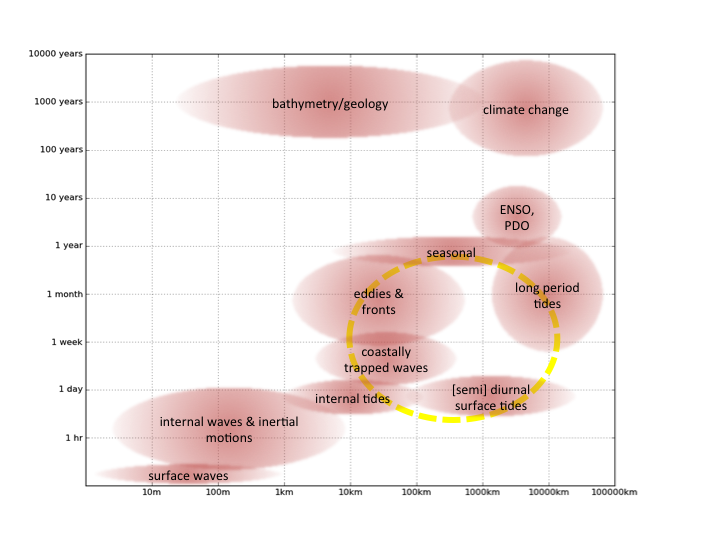
\includegraphics[width=130mm]{figures_2/ocean_scales.png}
\caption{Schematic indication of time/length scales of ocean processes.  The approximate scale limits for this research are highlighted. (Following \citet{Chelton:2001ws} )}
\label{fig:SCALES}
\end{center}
\end{figure}

`Sea level' is the elevation of the ocean/air interface at a place; though careful definitions are context dependant.  Elevation implies a reference datum and direction which can in fact present non-trivial and important issues.   Figure \ref{fig:SEALEVEL} indicates the relative nature of sea level without explicitly specifying the many nuances. \\
A well-defined sea surface is taken to be unproblematic.  Phenomena that may complicate the definition of sea level such as sea-spray, foam and debris will here be relegated to the category of noise.\\




The privileged role sea level plays in ocean forecasting can at least partly be attributed to it's \emph{observability}; and subsequently to fact that it has long been systematically recorded.  Collectively referred to as tide gauges, a variety of insitu sea level instruments are continuously operated in thousands of locations around the globe.   Tide gauges and tide gauge data have a thoroughly embedded role in ocean forecasting and a diversity of derived end-uses; including cadastral and commercial applications \cite{Level:2011wu}.\\
Away from the coasts sea level is of less direct economic interest, but open ocean sea level is in fact very significant.  One reason for this importance pertinent to operational oceanography is that sea level can be remotely observed and provides insight into physical state of the full water column; whereas observations of the ocean interior are extremely sparse.
\begin{quote}
Observations of the surface topography - together with complementary in situ observations\dots{}- are central to understanding the dynamics of the global oceans \citep{Wilson:2010hy}.
\end{quote}




Looking more closely there are in fact multiple sea level quantities in use operationally; even within the observational record.
For instance, tide gauges observe sea level relative to an land-fixed structure over a few square centimetres; and are commonly constructed to physically filter wind waves.  Simultaneously, satellite altimetry systems deliver geocentric Sea Surface Height (SSH) and Sea level Anomaly (SLA) quantities based on returns from a spatial footprint orders of magnitude larger. \\

\begin{figure}[!h]
\begin{center}
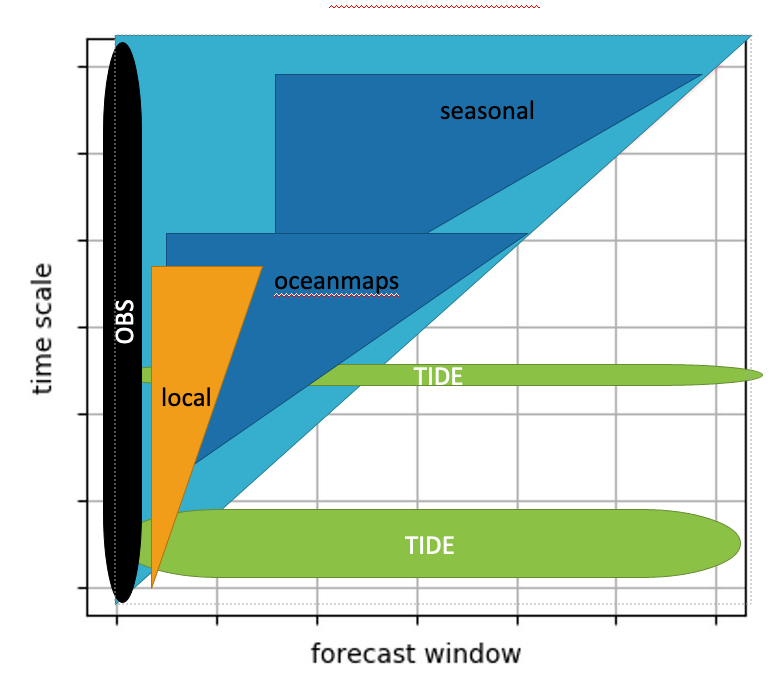
\includegraphics[width=120mm]{figures_2/sealevel_cartoon.png}
\caption{Simplified illustration of the relative nature of sea level and different observing platforms.}
\label{fig:SEALEVEL}
\end{center}
\end{figure}



Figure \ref{fig:SPECTRA_EG} illustrates spectra of sea level variation derived from coastal tide gauge time-series.  Coastal sea level is typically described as an example of a `mixed spectra' \citep{Percival:1998tw}, in the sense the signal can be viewed as a combination of discrete spectral lines embedded in a background continuum of coloured noise.  For the purposes of this introduction, the overall `redness' of the spectra and the prominence of spikes at tidal frequencies is highlighted.\\

%\begin{figure}[h]
%\begin{center}
%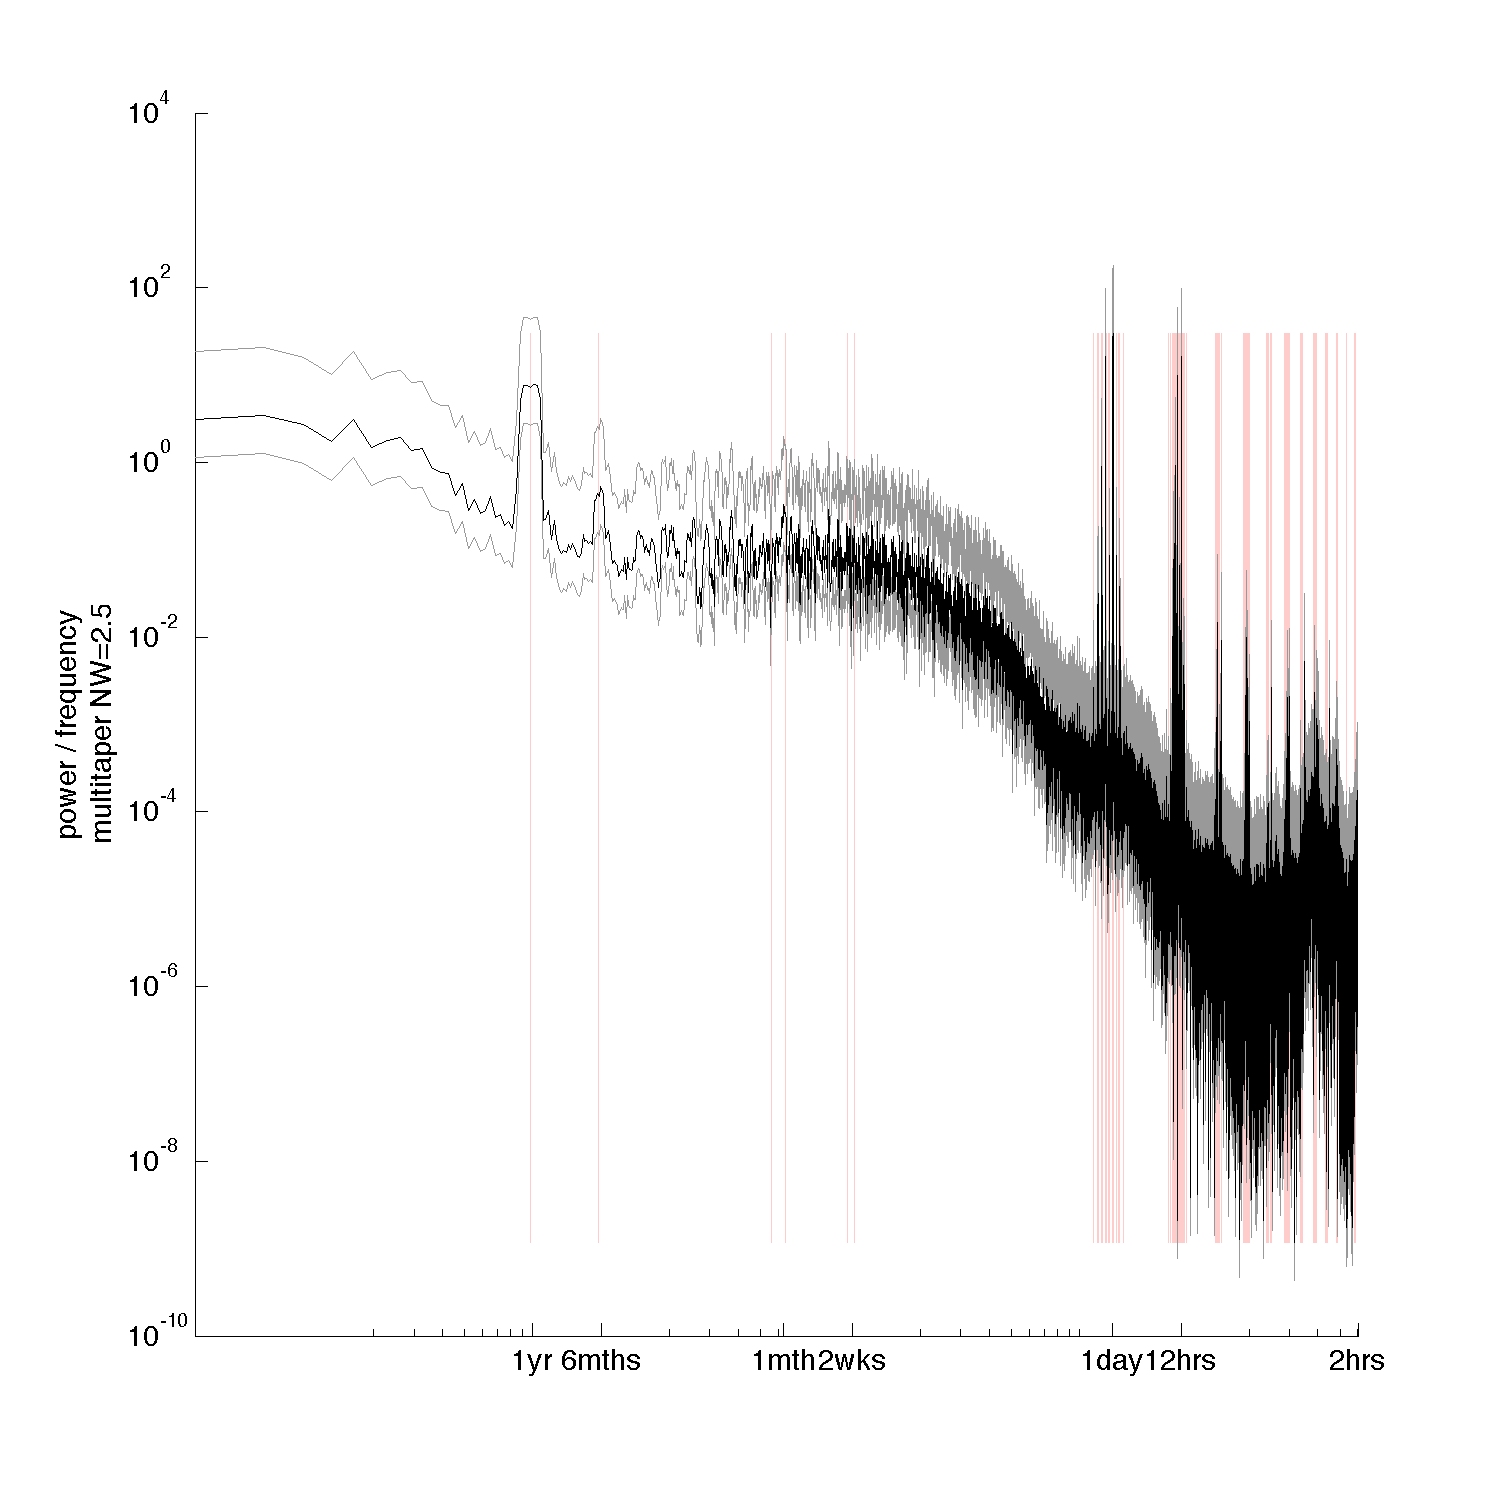
\includegraphics[width=120mm]{figures_2/spectra_109504.png}
%\caption{Example sea level spectra - illustrative of a red background continuum with distinct peaks.}
%\label{fig:SPECTRA_EG}
%\end{center}
%\end{figure}



\begin{figure}[!h]
	\centering
	\subfloat[Darwin in Northern Australia - large diurnal tide.]{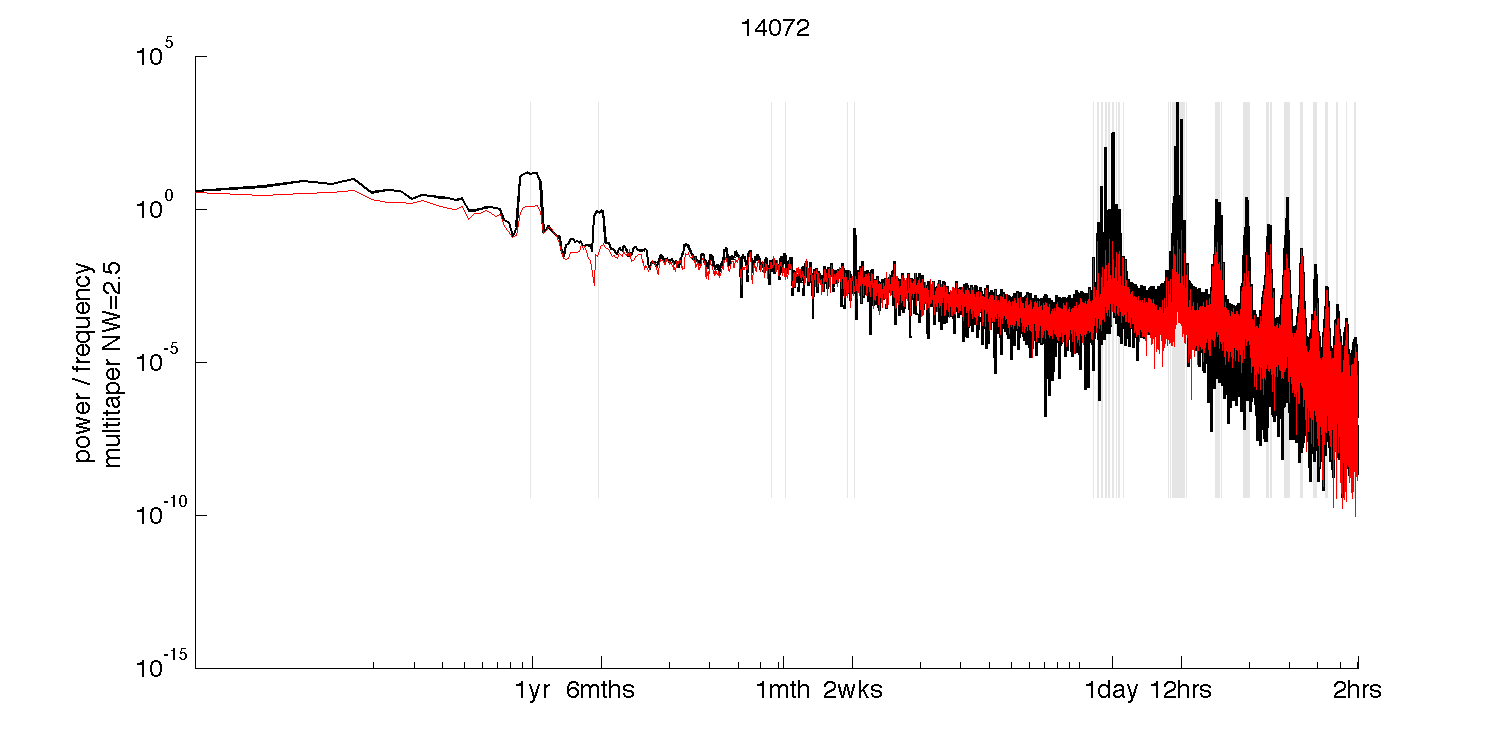
\includegraphics[width=130mm]{figures_2/plot_14072.png}} \\
	\subfloat[Esperence in Southern Australia - powerful synoptic signal.]{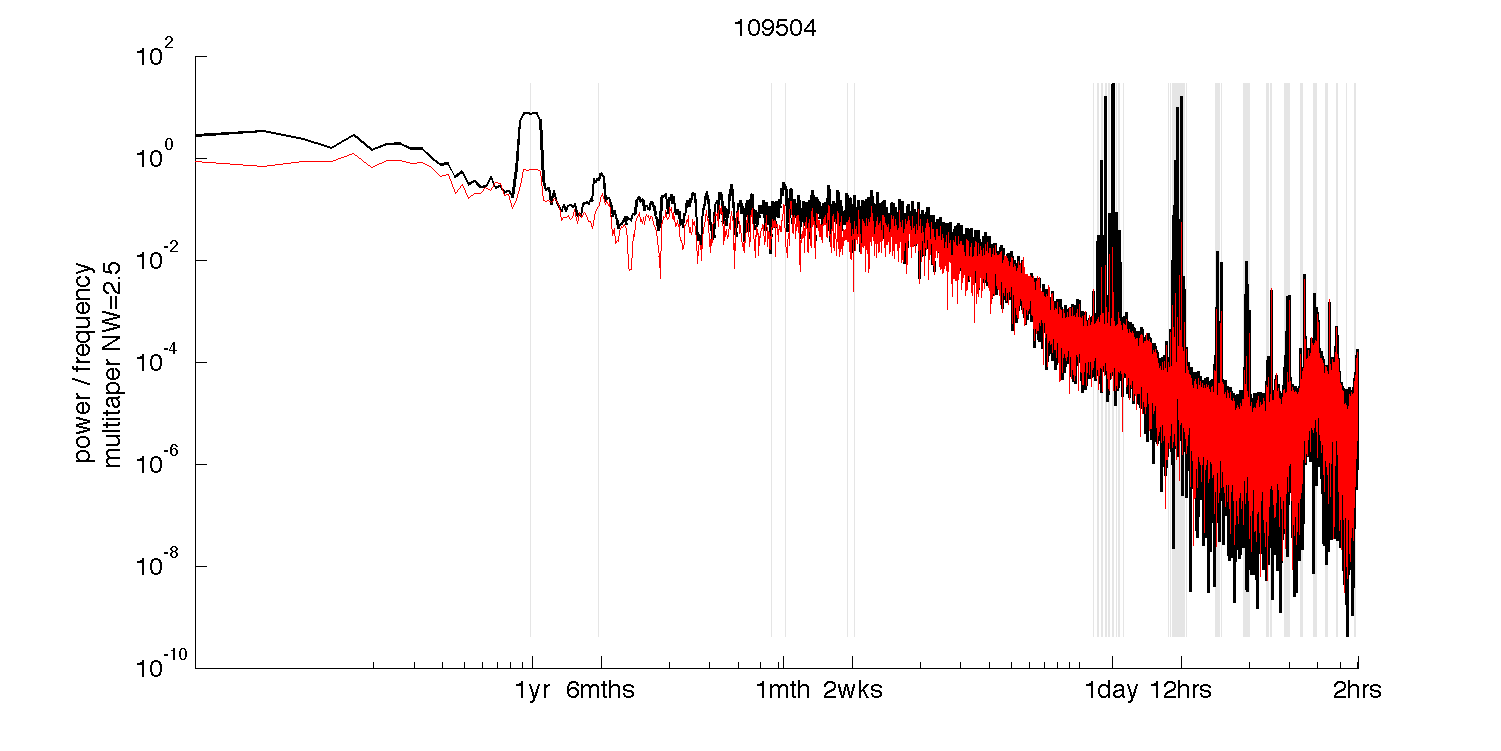
\includegraphics[width=130mm]{figures_2/plot_109504.png}}
	\caption{Spectral estimates for timeseries of hourly data at coastal tide gauges.   Black = observations, Red = Residual compared to official harmonic tidal analysis. }
    \label{fig:SPECTRA_EG}
\end{figure}



